\documentclass{article}
\usepackage{graphicx}
\usepackage{amsmath} 
\usepackage{amssymb}
\usepackage{float}
\usepackage{algorithm}
\usepackage{algpseudocode}
\usepackage{subcaption}
\usepackage{multirow}
\usepackage{xcolor}
%--------- litteratur
\usepackage{natbib}
%---------- 

%---------- hyperref til hyperlink af litteratur
\usepackage[colorlinks=true, linkcolor=blue, citecolor=blue, urlcolor=blue]{hyperref}
%-----------

\title{Bachelor Project 2025}
\author{Navn 1 & Navn 2}
\date{June 2025}
% --------- Fodnoter og litteratur ------

% -------- fodnoter og litteratur -------

\begin{document}
\maketitle
\pagenumbering{roman}
\setcounter{page}{1} 

\newpage
\section*{Abstract}



\newpage
\tableofcontents
\newpage

\pagenumbering{arabic} % Sets page numbering to arabic (1, 2, 3, ...)
\setcounter{page}{1} 

\section{Introduction}

\section{Economic Theory}
HAL R. Varian "Intermediate Microeconomics with calculus"
\newline 
The “Cournot-Bertrand Debate”:
A Historical Perspective 
https://competitionandappropriation.econ.ucla.edu/wp-content/uploads/sites/95/2020/12/CournotBertrand-debate.pdf
Jean Magnan de Bornier 
\newline
In the following section we will focus on unraveling the Economic theory behind the dynamics of the game we will be simulating. 
The overall idea is that we are using machine learning to simulate price competition between two firms. This is being done using a reinforcement learning algorithm known as Q-learning in a duopoly setting known from a Bertrand economy. This framework is based on an article from \cite{Klein2021}, who uses the work of \cite{MaskinTirole} as the economic base for the model. Therefore it is a dynamic, sequential setting, where the firms will take turns of setting their price.
Like \cite{Klein2021}, we will investigate whether using algorithmic pricing can lead to, what can be seen as collusive behaviour.
\newline
We are investigating the dynamics of the game and specifically what happens when you change the number of prices that each firm can set.
\newline



\subsection {Game Theory}
\label{GameTheory}
Game theory, broadly speaking, is a way to provide a framework for trying to understand how rational agents make decisions in individual and group settings, when agents' payoffs depend on their own and other choices.(TADELIS)
\newline
The framework of the simulations in our project are based on game theory. Therefore, we will now introduce project-relevant definitions from game theory and assumptions which will be used when setting up our simulations.
\newline
First off, agents (or players), will be referred to as firms, and are assumed to be rational, meaning that they act according to the actions which maximizes their payoff (TADELIS). The firms' objective is therefore to maximize profits.
\newline
Firms can choose to set different prices when playing against each other. Thus, setting prices are the actions that the firms can take.
The set of actions is called a 'strategy', when we analyze the setting from a game theory perspective. With different strategies, we can end up with different equilibria.
\subsubsection{Nash Equilibrium, SPNE and MPE}
A \textbf{Nash equilibrium} is a strategy or set of strategies in a game where no agent has any incentive to deviate from their strategy, given what the other agents are playing. This ensures that in equilibrium, each agent's strategy is a best response to the other's (\cite{tadelis}).
\newline
In our simulation we are playing a repeated game, which leads us to the definition of the Subgame Perfect Nash Equilibrium (SPNE). A SPNE is a refinement of the Nash equilibrium and means that every subgame of the game is a Nash equilibrium \citep[p. 157]{tadelis}. 
\newline
In a dynamic game like ours, the number of possible subgames is very large. To simplify analysis, \cite{MaskinTirole} introduced the concept of a \textbf{Markov-perfect equilibrium (MPE)} which will be further explained in section \ref{economic Environment}. 


\subsection{Bertrand competition}
The overall competition framework used in the project, will be based on the ideas of Joseph Louis François Bertrand. In a market for a homogeneous good, sold by symmetric firms, Bertrand came up with the theory, that the firms will only be setting the price while the market then will be determining the quantity sold(VARIAN). Bertrand's logic can be used on oligopolies, but as Bertrand originally framed his arguments in 1883 (Jean Magnan De Bornier), this project will be in the setting where only 2 firms exist on the market, namely duopoly. 
\newline
The reasoning for choosing our setting as a duopoly follows from the settings of \cite{MaskinTirole} and thereby \cite{Klein2021}. The ideas of price cycles such as Edgeworth cycles or the case of focal pricing, are described for two firms. Therefore, it is sensible that our setting is also based on two firms, such that we can analyze the dynamics that arises from our model.
Furthermore, we are investigating the dynamics of what happens when we change the number of price points, meaning the number of different prices that the firms can set (will be referred to as the parameter \textit{k}). It is therefore computationally heavy when you introduce more than two firms in the simulation, as the computations needed to be done rises with the parameter \textit{k}.  
\newline
Bertrand originally showed that under all the assumptions above and an assumption of constant cost, the Bertrand equilibrium is when the price is equal to the marginal cost, which is also a Nash equilibrium. However, in markets with few sellers, firms do not typically sell their goods at the marginal cost. 
\cite{MaskinTirole} partly blame this on the fact that the original model proposed by Bertrand was static, meaning that both firms set their prices simultaneously without knowing what the other firm set as a price, and the market clears and the game ends. They argue that having a dynamic model may be important to capture the dynamics of actual price competition (\cite{MaskinTirole}).
In a dynamic model, firms set prices in multiple rounds. This is important for us, as we are investigating the dynamics of price competition.  
\newline
As mentioned before, our model is a dynamic and sequential. \cite{Klein2021} argues that a sequential dynamic model is a more realistic model to capture pricing competition from the real world.
Other researchers, such as \cite{Calvano} have used a simultaneous dynamic setting, where firms play a repeated game, but set their prices in each turn at the same time. We believe that the sequential dynamic setting used in \cite{Klein2021} is more representative of the real world, as it is unlikely that firms always would set prices on the same goods, at exactly the same time. In a duopoly, it's more realistic to assume that one firm sets its price first, the second firm then observes this and sets its own price in response, and finally, the first firm adjusts its price again based on the second firm's price.





\subsection{Economic environment}
\label{economic Environment}
Our model, which is based on \cite{Klein2021}'s sequential pricing duopoly, uses Q-learning in a simulation setting, which we will also do.
We will now further describe the economic environment, which is based on the work of \cite{Klein2021}. 
\newline
Two firms, \textit{i} and \textit{j} take turns on setting prices in infinitely repeated discrete time indexed by $t = \{1,2,3,... \} $. Thus, firm \textit{i} sets price $p_{i,t}$ and firm \textit{j} sets the price $p_{j,t}$ in period \textit{t}. 
The prices that the firms can choose are discrete, evenly spaced and between 0 and 1. The number of different prices that the firms can set are determined by \textit{k}, such that the price interval is denoted by $P = \{0, \frac{1}{k}, \frac{2}{k}, \frac{3}{k},...,1\} $. Prices are set sequentially, such that in even time periods firm $p_i$ sets their price, and in odd time periods $p_j$ sets their price.
\newline
Assuming no marginal or fixed costs, the profit function for firm \textit{i}, in time period \textit{t} is described as:
\begin{equation}
    \pi_i (p_{it},p_{jt}) = p_{it}D_{it}(p_{it},p_{jt})
\end{equation}
where $p_{jt}$ is the price of the opposite firm, and $D_{it}$ is the demand as a function of its own price $p_{it}$, and the price of the opposing firm, $p_{jt}$.
Firms discount future profits with $\delta \in [0,1)$, such that it is the objective of each firm to maximize, at time \textit{t}, the following:
\begin{equation}
\max\sum_{s=0}^{\infty}\delta^s\pi_i(p_{i,t+s},p_{j,t+s})
\end{equation}
\newline
The demand function is defined as:
\begin{equation}
D_i(p_{it},p_{jt}) =
\begin{cases}
  1-p_{it} &\text{if } p_{it} < p_{ij},\\
  \frac{1-p_{ij}}{2}   & \text{if } p_{it} =p_{ij},\\
  0   & \text{if } p_{it} > p_{ij}
\end{cases}
\end{equation}
Which means that the firm with the lower price takes the whole market. If both firms set the same price, they split the market evenly. 





The monopolist's profit corresponds to the joint-profit maximizing profit. Therefore, we calculate the monopolist's profit, such that it can later be used as a benchmark. This allows for a clearer interpretation of the profit levels observed in the simulation, by comparing them to the theoretical maximum achievable profit through full cooperation.
\newline
The monopolist's demand function is:
\begin{equation}
    D(p) = 1-p
\end{equation}
with a profit of
\begin{equation}
    \pi (p) = p \cdot D(p) = p \cdot (1-p) \Leftrightarrow \pi (p) = p - p^2
\end{equation}
maximizing over p, we take the derivate with respect to p: 
\begin{equation}
    \cfrac{d \pi(p) }{d p} = 1-2p
\end{equation}
and now setting the equation equal to 0 and isolate for p:
\begin{equation}
    0 = 1 - 2p \Leftrightarrow p = \cfrac{1}{2}
\end{equation}
Which means that the joint-profit maximizing price is:
\begin{equation}
    p^M = 0.5
\end{equation}
with a profit for each firm of:
\begin{equation}
\label{MonopolistPrice}
\pi_{ij}^M (p^M) = 0.5 \cdot \cfrac{1 - 0.5}{2} = 0.125
\end{equation}
\label{Joint_profit_price}
\newline
Following the works of \cite{Klein2021} and \cite{MaskinTirole}, we impose the Markov assumption: only directly relevant payoffs are used to determine the strategy of the firms. This means that the strategy that the firms follow, are only dependent on the price that the other firm set in the last period $p_{j,t-1}$. This implies that the history of the prices (other than the last period) are irrelevant, and that there is no communication between the firms.
As mentioned in section \ref{GameTheory}, strategies are the prices that the firms are setting.
\newline
Because we are in a dynamic environment, we will define what will be an equilibrium in this setting. 
The following value function is a Nash equilibrium for all prices along the equilibrium path, if the condition holds for both firms:
\begin{equation} \label{KleinBellmanEq}
    V_i(p_{jt}) = \mathop{\text{max}}_{\text{p}} [\pi_i (p,p_{jt}) + E_{p_{j,t+1}}[\delta \pi_i (p,p_{j,t+1})+\delta^2 V_i (p_{j,t+1}) ]]
\end{equation}
Equation (\ref{KleinBellmanEq}) is written in the style of \cite{Klein2021}, who has the equation from \cite{MaskinTirole}. They introduce the concept of a Markov Perfect Equilibrium (MPE). An MPE is a special type of SPNE where the strategy of each player depends only on the current “state” of the game — not the full history. This is known as the \textbf{Markov assumption}, and in our model, the state is simply the price set by the opponent in the previous round.
If you include off-equilibrium prices, for all prices a strategy pair $(R_1,R_2)$ is MPE if equation (\ref{KleinBellmanEq}) holds.

\subsubsection{Edgeworth Price Cycles and Focal Pricing} \label{EdgeworthFocalpricingSec}
Further, \cite{MaskinTirole} show that if firms value future profits sufficiently \footnote{When \cite{MaskinTirole} talk about valuing future profits 'sufficiently' high with a 'sufficiently' high discount factor, $\delta$, they mention one close to 1, without giving a specific number. \cite{Klein2021} uses a $\delta$ value of 0.95.}, two kinds of MPE's exist, 
namely focal pricing and Edgeworth price cycles.
Focal pricing is when both firms are playing the same price, repeatedly. This equilibria exists because of the fear from the firms, that if they undercut their competitor, that the competitor would follow suit and undercut them aswell. This would start a price war, which would be costly for the firms. And because they value future profit sufficiently, none of the firms are willing to start this price war. Similarly, the firms are not willing to increase the price, as they believe that the other firm would not follow, and then they would lose the entire market.
\newline
Edgeworth price cycles are when firms gradually undercut each other, to increase market share, until the price war becomes too costly, and one of the firms resets the price to a 'high' price, and the undercutting begins again (\cite{MaskinTirole}). In this way, a cycle pattern arises, which an example of can be seen in Figure \ref{fig:EdgeworthCycle}.

\begin{figure}[H]
    \centering
    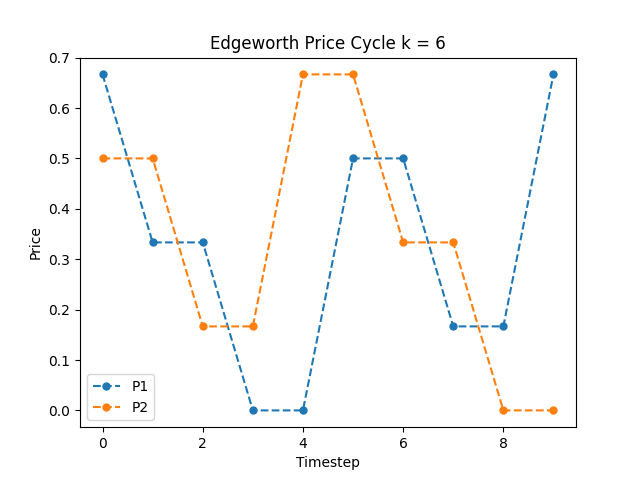
\includegraphics[scale = 0.75]{Edgeworth price cycle k = 6.png}
    \caption{The most competitive Edgeworth price cycle for two firms with \textit{k} = 6. Firms undercut each other until the first firm to observe the lowest price resets the price cycle. In this case firm 2 are the first to reset the cycle, and then the next reset is done by firm 1.}
    \label{fig:EdgeworthCycle}
\end{figure}
The most competitive Edgeworth cycle is used as a benchmark for the competitive level in the article by \cite{Klein2021}. It is defined as an Edgeworth cycle where the firms undercut each other by one increment at a time until they reach marginal cost, which is 0 in our case. Then the first firm to observe the price at marginal cost, resets the price to one increment above the monopoly price, and the undercutting begins again.
The most competitive Edgeworth price cycle changes, as the price interval changes (number of prices that the firms can set, denoted by parameter \textit{k}). This is important to note, as we will later analyze what happens when \textit{k} changes. 
\newline
We simulate the most competitive Edgeworth cycles for different values of \textit{k} in Python, and calculate the per period profit.
The per period profit of the most competitive Edgeworth price cycle will serve as a benchmark for the competitive level of profit, just as it does in \cite{Klein2021}. The profits can be seen in Table (\ref{tab:kPrPeriodProf}).
\begin{table}[H]
    \centering
    \begin{tabular}{|c|c|}
        \hline
       \textit{k} & Per period profit of the 
 most competitive Edgeworth cycle \\
        \hline
        6 & 0.0611 \\
        \hline
        12 & 0.0699 \\
        \hline 
        24 & 0.0758 \\
        \hline
        48 & 0.0793 \\
        \hline
        100 & 0.0813 \\
        \hline
    \end{tabular}
    \caption{The per period profit associated with the most competitive Edgeworth price cycle for different values of \textit{k}.}
    \label{tab:kPrPeriodProf}
\end{table}

Note that other candidates for the competitive benchmark are the static Nash outcome of the game where both firms set the price at the marginal cost (or one increment above the marginal cost), both of which is a static Nash equilibrium. However, due to the dynamics of the game, the static Nash outcome is not a suitable benchmark for a repeated game (\cite{Klein2021}).

\section{Reinforcement learning theory} \label{ReinforcementLearningTheory}

\subsection{Introduction to Reinforcement Learning}
Reinforcement learning (RL) is a concept from machine learning, that differs from other types such as supervised learning and unsupervised learning.
Supervised learning is where you have labeled input-output pairs, and the objective is then to find the unknown function which this data is from. An example of supervised learning could be the very well-known OLS regression which tries to fit a linear model to data. In unsupervised learning, you have access to unlabeled data, and the objective is to find patterns or structures. An example of unsupervised learning could be K-means clustering which tries to find clusters in unlabeled data, thereby finding patterns. RL differs from these methods, and instead learns the most optimal choices through repeated interactions with the environment. This is therefore a 'trial and error' approach, where the algorithm tries new actions, and learns through which actions give the best rewards. A great and relevant example of an RL algorithm would be Q-learning \citep[p. 19-21]{marl-book}.
\newline 
\newline
A more general definition of RL by \cite[p. 20]{marl-book} is where they define RL as algorithms that learn solutions for sequential decision processes via repeated interaction with an environment.
From the definition it is clear where RL get its "trial and error" reputation. 
\cite{marl-book} will also serve as a primary source for this theory section and corresponding subsections.
\newline
A sequential decision process is when an agent inside an environment makes decisions and observes one time step at the time. To define sequential decision processes, a decision process model is needed to guide the decisions, and a learning objective must be established to evaluate each strategy. Together, the model and objective constitute a reinforcement learning problem, as shown in Figure \ref{fig:MARLside20} \citep[p. 20]{marl-book}). In relation to our thesis, we use Markov Decision Processes (MDP) as the decision process model for our Q-learning implementation.
\newline 
\newline
The environments in which we implement our RL algorithms determine whether we are dealing with Multi-Agent RL or Single-Agent RL. The two concepts of Single and Multi-agent RL will be elaborated upon later, but to quickly summarize: Single-agent RL interacts with an environment alone, while  Multi-agent acts with an environment with other agents\citep[p. 19-21]{marl-book}.
In this section, we will unpack the theory essential to understanding the underlying principles of Q-learning, beginning with the single-agent framework and MDP, trying to translate the general Q-learner setup to our Economic environment. 
\begin{figure} [H]
    \centering
    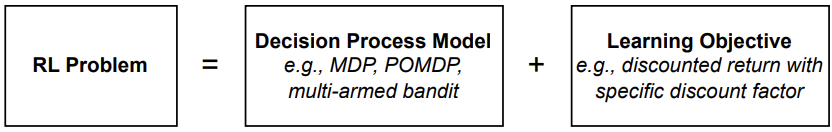
\includegraphics[width=0.5\linewidth]{MARLside20.png}
    \caption{Figure from \citep[p. 19-21]{marl-book} }
    \label{fig:MARLside20}
\end{figure}
\subsection{Single Agent Reinforcement Learning}
\subsubsection{Markow Decision Processes}
As metioned earlier, Markov Decision Processes (MDP) will be the Decision Process Model that we will focus on. It serves as the standard model for sequential decision processes that lays the foundation for
defining Single-Agent RL \citep[p. 19-22]{marl-book}. This can be said in more intuitive terms: MDP provides a structured way to model the process where an agent must make a series of decisions over time in an environment.
\newline
\textbf{Definition 1: Markov Decision Process \citep[p. 22]{marl-book}} A Discrete (MDP) consists of:
\begin{enumerate}
    \item \textbf{Finite set of states \( S \)}, with a subset of terminal states \( \bar{S} \subset S \).
    \item \textbf{Finite set of actions \( A \)}.
    \item \textbf{Reward function \( \mathcal{R}: S \times A \times S  \to \mathbb{R} \)}.
    \item \textbf{State transition probability function \( \mathcal{T}: S \times A \times S \to [0, 1] \)} such that
    \[
    \forall s \in S, a \in A : \sum_{s' \in S} \mathcal{T}(s, a, s') = 1 \quad 
    \]
    \item \textbf{Initial state distribution \( \mu: S \to [0, 1] \)} such that
    \[
    \sum_{s \in S} \mu(s) = 1 \quad \text{and} \quad \forall s \in \bar{S}, \mu(s) = 0 \quad 
    \]
\end{enumerate}
Let us now try to explain exactly what this mean starting with the first item of the definition.
\newline 
\textbf{Finite set of state S} represents all the possible situations an agent can be in. In our case, a firm's state is determined by the price set by its competitor. Instead of defining specific terminal states, where the agent stops acting, we ensure that the simulation ends by imposing a maximum number of time steps, which serves the same purpose and is the approach we use in our simulations.
\newline
A \textbf{Finite set of actions A} are the possible actions that an agent would have. In our case this is the firm's different options for setting the price, which is determined by the parameter \textit{k}. 
\newline
The \textbf{Reward function} determine the reward of an action and thereby how well the action was guiding the agent. In our case, this will be a profit function. 
\newline
The \textbf{State Transition probability function's} goal is to explain how the environment changes. It can be thought of like a rulebook, containing rules of the game. The state transition probability function only have a theoretical relevance to this thesis, which will be made clear in section \ref{Temporal Difference Learning and Q-learning}. 
\newline
The \textbf{Initial State Distribution} defines the probabilities of the agent being in a particular state at the beginning of the game. For example, if a firm has two possible starting states $s_1$ and $s_2$ (which would be determined by a \textit{k} value of 2), the initial state distribution might look like $s_1=30\%$ and $s_2 = 70\%$ meaning there's a $30\%$ chance the firm starts in state $s_1$ and a $70\%$ chance it starts in state $s_2$.
\newline 
\newline 
One could easily think that the Markow Decision process could have something to do with the Markow assumption, also known as the Markow property mentioned in section \ref{GameTheory}, and indeed it does. 
As we know, the Markow assumption says that the future state (competitor price) and reward (profit) are conditionally independent of past states (competitor prices) and actions (own prices), when you have the current state (competitor price) and action (own price). Mathematically the assumption is expressed in equation \ref{Markow_property}.
\begin{equation}
\label{Markow_property}
P(s_{t+1}, r_t | s_t, a_t, s_{t-1},a_{t-1} \dots, s_0, a_0) = P(s_{t+1}, r_t | s_t, a_t)
\end{equation}
This allows us to only give an agent the current state and it would still be sufficient information for it to take optimal actions in an MDP\citep[p. 23]{marl-book}. 
Limiting the agent therefore limits the amount of complex coding and makes the process less computationally demanding, by not needing to store and use past states and actions.
\subsubsection{Value functions and Bellman equation}
Moving forward we will have to define a strategy function, that returns a probability from which the MDP chooses an action conditioned on the state. It will be denoted as: $\mathcal{P}(a_t,s_t)$. When working with MDP, one can define a solution a as optimal strategy $\mathcal{P}^*$, which is the strategy that results in the maximum expected discounted return. 
To determine which strategy does exactly this we will use the Bellmann Equation, also known as the state value function, which can be seen in equation (\ref{bellmann-equation})
\begin{equation}
    \label{bellmann-equation}
    V^{\mathcal{P}}(s)= \sum_{a\in A}\mathcal{P}(a|s)\sum_{s'\in S}\mathcal{T}(s'|s,a)[\mathcal{R}(s,a,s')+\delta V^{\mathcal{P}}(s')]
\end{equation}
Where s' denotes the future states and $\delta$ is the discounting parameter. 
The purpose of equation (\ref{bellmann-equation}) is to give the expected return when selecting actions with strategy $\mathcal{P}$, starting in state s. From the same logic, we can now define the action value function $Q^{\mathcal{P}}(a,s)$ in equation (\ref{action_value_func}).
\begin{equation}
    \label{action_value_func}
    Q^{\mathcal{P}}(a,s)=\sum_{s'\in S}\mathcal{T}(s'|s,a)[\mathcal{R}(s,a,s')+\delta\sum_{a'\in A}\mathcal{P}(s|a')Q^{\mathcal{P}}(a',s')]
\end{equation}
$Q^{\mathcal{P}}(a,s)$ returns the expected value but this time when  selecting an action a in state s and then following strategy $\mathcal{P}$ to select actions afterwards.
Since we are in the MDP, the strategy is optimal if its corresponding value function is optimal. This then leads us to Bellman Optimality Equations which can without needed reference to the strategy functions because...., where * denotes optimality:
\begin{equation}
    \label{V_optimal}
    V^*(s) = \max_{a\in A}\sum_{s'\in S}\mathcal{T}(s'|s,a)[\mathcal{R}(s,a)+\delta V^*(s')]
\end{equation}
\begin{equation}
    \label{Q_optimal}
    Q^*(s,a)= \sum_{s'\in S}\mathcal{T}(s'|s,a)[\mathcal{R}(s,a,s')+\delta \max_{a'\in A}Q^*(s',a')]
\end{equation}
Equations \ref{V_optimal} and \ref{Q_optimal} illustrates that the optimal strategy in an MDP relies on the optimal value function. To find the optimal strategies for given states, we select actions that maximize the value, as shown in equation \ref{Optimal_strategy}.
\begin{equation}
    \label{Optimal_strategy}
    \mathcal{P}^*(s) =  \arg \max_{a \in A}Q^*(s,a)
\end{equation}
Two families of algorithms are used to calculate optimal value functions and thereby optimal strategies, respectively Dynamic programming and Temporal Difference learning. While Dynamic Programming estimates value functions using complete knowledge of the MDP, Temporal difference learning updates value estimates based on interactions with the environment, making the latter of relevance to Q-learning and by extension our thesis. 
\citep[p. 26-28]{marl-book}
\subsubsection{Temporal difference Learning and Q-learning}
\label{Temporal Difference Learning and Q-learning}
Temporal difference learning (TD) is a family inside the world of RL where value functions and optimal strategies are learned through experiences which are generated in the following loop: An agent choose an action, to which the environment responds by modifying the state, which the agent then observes through a reward function and responds to by choosing an action. In the following, the reward function $\mathcal{R}(s^t,a^t,s^{t+1})$ will simply be denoted as $r^t$. As mentioned above, TD learning relies on interactions with the environment and does not require full knowledge of the Markov Decision Process. This makes the state transition function redundant for the equations. As a result, we can modify the Bellman optimality equations, originally shown in equations (\ref{V_optimal}) and (\ref{Q_optimal}) to the equations (\ref{TD_V_optimal}) and (\ref{TD_Q_optimal}).
\begin{equation}
    \label{TD_V_optimal}
        V^*(s) = \max_{a\in A}[r^{t+1}+\delta V^*(s^{t+1})]
\end{equation}

\begin{equation}
    \label{TD_Q_optimal}
        Q^*(s,a)= [r^{t+1}+\delta \max_{a'\in A}Q^*(s^{t+1},a')]
\end{equation}
In temporal difference learning, the update rule for learning the action value function $Q(s,a)$, uses equation (\ref{TD_Q_optimal}) and is shown in equation (\ref{TD_update_Q}) just below. 
\begin{equation}
    \label{TD_update_Q}
    Q(s^t,a^t)\leftarrow Q(s^t,a^t)+\alpha *[\underbrace{ r^{t+1}+\delta \max_{a'\in A} Q(s^{t+1},a')}_{\text{Equation \ref{TD_Q_optimal}}}-Q(s^t,a^t)]
\end{equation}
The update rule (equation (\ref{TD_update_Q})) is used to estimate the action value function after interactions with the environment on a given time. 
In the update rule, a new variable $\alpha$ is used, which is the learning rate, also known as step size which lies between the values (0;1]. It can be seen as how much new interactions are weighted against older interactions. Using the theory from above we can now introduce pseudocode for the single agent Q-learning algorithm, showcased Algorithm 1, which uses the update rule from equation (\ref{TD_update_Q}).
\begin{algorithm}[H]
\caption{Q-learning for MDPs using the Epsilon Greedy Strategy Method}
\begin{algorithmic}[1]
\State Initialize: \( Q(s, a) = 0 \) for all \( s \in S, a \in A \)
\State Repeat for every episode:
\For{$t = 0, 1, 2, \dots$}
    \State Observe current state \( s^t \)
    \State With probability \( \epsilon \): choose random action \( a^t \in A \)
    \State Otherwise: choose action \( a^t \in \arg \max_{a} Q(s^t, a) \)
    \State Observe own reward \( r^{t+1} \) and next state \( s^{t+1} \)
    \State \( Q_i(s^t, a^t) \gets Q(s^t, a^t) + \alpha [r^{t+1} + \delta \max_{a} Q(s^{t+1}, a) - Q(s^t, a^t)] \)
\EndFor
\end{algorithmic}
\end{algorithm}
Epsilon-Greedy Strategy Method is a way to making sure the Q-learner explores the action-state space, while still converging to an optimal strategy. The method is shown down below in equation (\ref{epsilongreedy}) 
\begin{equation}
    \label{epsilongreedy}
    a^t\begin{cases}
        \sim\text{U}(A)& \text{with probability $\epsilon^t$}\\
        \arg \max_a Q(s,a) & \text{with probability 1-$\epsilon^t$}
    \end{cases}
\end{equation}
It shows how an action is chosen with a probability determined by $\epsilon$ to either pick a random action from a uniform distribution or an action that maximize the action-value function $Q(s,a)$. This is what happens at line 5-6 in algorithm 1. 
The purpose is to gradually decrease the value of epsilon as the number of time steps increases, reducing the likelihood of exploration over time and making sure that the Q-learner eventually converges toward a strategy \citep[p. 32-35]{marl-book}.
\subsection{Multi Agent Reinforcement Learning}
Now that the section above have given a better understanding of the theory and methods behind how Single-Agent RL works, we will now move onto Multi-Agent RL. The relevance of both having multi agent and single agent RL theory and methods will become clear in the following. Figure \ref{fig:marside44} from \citep[p. 44]{marl-book} finely illustrates an overview of the Multi-agent RL hierarchy. It illustrates how Repeated Normal-Form games and Markow Decision Processes are special cases of Stochastic Games which are special cases of Partially Observable Stochastic Games. The figure also shows that the number of states and agents classify each type of game. In this thesis we are focusing on Q-learning and Q-learners (agents) playing and learning against each other. The states will be fully observed and transparent for each agent and combining that with having multiple agents working in the same environment means we only will be exploring the Stochastic Games and Markow decision processes.
\begin{figure}[H]
    \centering
    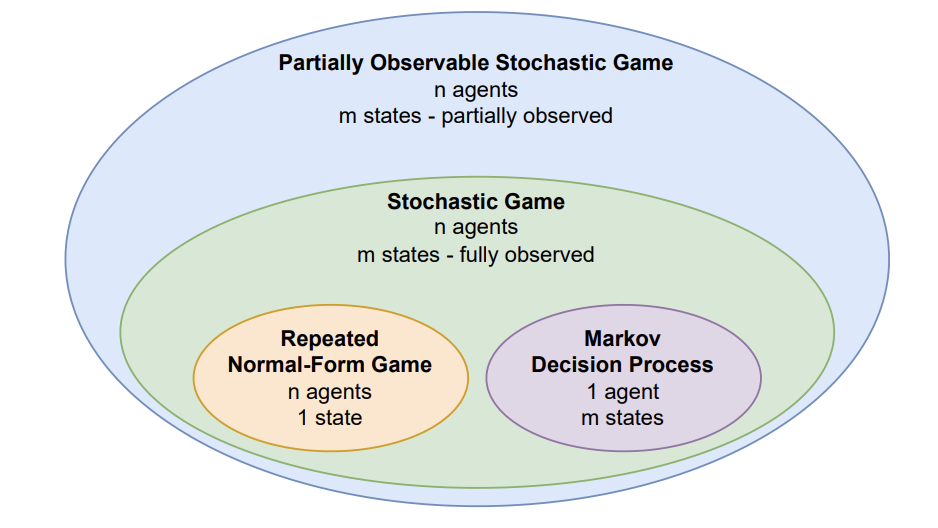
\includegraphics[width=0.5\linewidth]{Multi-agent-figure.png}
    \caption{Multi-Agent RL Hierarchy }
    \label{fig:marside44}
\end{figure}
\subsubsection{Stochastic games and Independent Learning}
Most of the theory that Stochastic games are build upon is very similar to MDP's and therefore to avoid repeating ourselves the following will seem more superficial. A more formal definition of a stochastic game can be seen in appendix \ref{stochasticgamedef}. 
\newline
The definition of a stochastic game is just an expansion of the definition (1) of the MDP, with the addition, that it can handle multiple agents in the same environment. This is handled by introducing indices. In our thesis the number of agents (firms) will, as mentioned, be 2. Similar to the MDP, the Stochastic games have the same Markow Assumption as shown in equation \ref{Markow_property}. Given these similarities, it comes as no surprise that Stochastic Games are also referred to as Markov Games. \citep[p. 48]{marl-book}.
\newline 
\newline
Multi-agent RL can be used to learn strategies for handling real-world problems. And since the problems that RL are used to solve differs quite a bit, the approach on how to actually apply the RL also differs quite bit. In this thesis, we will be using the approach of reducing 
a multi-agent RL game into multiple single-agent RL games within the Multi-agent game. This is a standard approach in RL which lowers complexity by reducing the multi-agent learning problem to a single-agent learning problem. More specifically there are 2 different ways to execute this approach, namely Central Learning and Independent Learning. Central Learning is when you take the joint action space for multiple agents and then apply single Agent RL to the joint actions space all together, therefore learning a central strategy that chooses actions for all agents. Central Learning could therefore make sense to use in environments where the agents work together. An example of this could robot lawn mowers working together to learn how to cut a field of grass most efficiently. Independent Learning is when you apply single agent RL to each agent independently, essentially isolating each agent. This means that each agent learns their own independent strategies and ignore the presence of the other agents\citep[p. 95]{marl-book}. They just see the other agents as part of the environment. Independent learning would therefore be a great approach for environments where agents work against each other, which is why this is the approach we have been using in the thesis, as the firms will be competitors. 
\newline
\newline
The independent Learning approach to multi-agent RL brings us to the pseudo code for Independent Q-learning seen in Algorithm 2 \citep[p. 98]{marl-book}, which is easy to recognize, as it is just an expansion of Algorithm 1. The new thing is again that indices have been introduced to handle multiple agents and their corresponding action and state space.
\begin{algorithm}[H]
\caption{Independent Q-learning (IQL) for stochastic games}
\textbf{Algorithm controls agent \(i\)}
\begin{algorithmic}[1]
\State Initialize: \( Q_i(s_i, a_i) = 0 \) for all \( s_i \in S_i, a_i \in A_i \)
\State Repeat for every episode:
\For{$t = 0, 1, 2, \dots$}
    \State Observe current state \( s_i^t \)
    \State With probability \( \epsilon \): choose random action \( a_i^t \in A_i \)
    \State Otherwise: choose action \( a_i^t \in \arg \max_{a_i} Q_i(s_i^t, a_i) \)
    \State (meanwhile, other agents \( j \neq i \) choose their actions \( a_j^t \))
    \State Observe own reward \( r_i^{t+1} \) and next state \( s_i^{t+1} \)
    \State \( Q_i(s_i^t, a_i^t) \gets Q_i(s_i^t, a_i^t) + \alpha [r_i^{t+1} + \delta \max_{a_i} Q_i(s_i^{t+1}, a_i) - Q_i(s_i^t, a_i^t)] \)
\EndFor
\end{algorithmic}
\end{algorithm}

\subsection{Linking to Economic Environment}
\label{siste Q teori afsnit}
As mentioned in section \ref{economic Environment} the game that we will be simulating in this thesis is between 2 firms. Firm \textit{i} and \textit{j} exist in a sequential duopoly following a bertrand economy, and are competing by setting prices.
By translating the RL theory to the Economic Environment, introduced in section \ref{economic Environment}, we will get the following action and state space and reward function, for firm \textit{i}, while it is symmetrical for firm \textit{j}:
$$A_i = P = \{0, \frac{1}{k}, \frac{2}{k}, \frac{3}{k},...,1\} \text{,  where }p_i\in P$$
$$S_i=P=\{0, \frac{1}{k}, \frac{2}{k}, \frac{3}{k},...,1\} \text{,  where }p_j\in P$$ 
$$\mathcal{R}(a_i,s_i) = \pi_i(p_i,p_j)$$
Therefore, the action space is all of the prices that the firm can set (determined by \textit{k}). The state space is determined by the competitor price, and the size of this space will also be given by \textit{k}. The reward function is determined by the profit function.
\newline
Algorithm 2 shows a way to implement Q-learning using independent learning. In this algorithm the firms are playing each other simultaneously, meaning that they in each time step both are setting a price. 
The decision process we want to simulate is turn-based, between firms since the firms will be taking turns in setting the price against each other as in \cite{Klein2021}. 
\newline 
Our simulations will therefore handle this variation of sequential turn-based setting using the following rewards definition inspired by \cite{Julius2023}, who also followed the work of \cite{Klein2021}: 
\begin{equation}
\label{last_reward}
    r_i^{t+1} = \pi_i(p^t_i,p^t_j) + \delta\pi_i(p_i^t,p_j^{t+1})
\end{equation}
The definition shown in \ref{last_reward} equation is tailored to this exact scenario. It takes into consideration that firm \textit{i} is never setting prices in 2 consecutive time steps, by defining its rewards as the direct profit and the profit in the next time step where a new state is introduced, when firm \textit{j} sets a price. $\delta$ discounts the future state profit for one period. Similarly, we also need to adapt the use of the action value function the same way giving us an update rule, which is a modification of equation \ref{TD_update_Q}:
\begin{align}
\label{Klein_update_rule}
Q(p_j^t,p_i^t)\leftarrow Q(p_j^t,p_i^t)+\alpha *[&r_i^{t+1}+\delta^2 \max_{p_i'\in p_i} Q(p_j^{t+1},p_i') -Q(p_j^t,p_i^t)], \\
&r_i^{t+1} = \pi_i(p^t_i,p^t_j)+\delta\pi_i(p_i^t,p_j^{t+1}) \notag 
\end{align}
Again, notice that the Q-value is now discounted for 2 time steps ($\delta^2$), again to handle the sequential turn-based setting.
\newline 
It is also worth noting the similarity between equation (\ref{Klein_update_rule}) and equation (\ref{KleinBellmanEq}). As noted by \cite{Klein2021}, this relationship comes from the fact that Q-learning, via recursive updating, aims to solve a dynamic programming condition. DERFOR ER EN LØSNING ALTID EN MPE  MÅSKE ?
\newline 
With this new update rule and corresponding game modification we will now show the last algorithm, which is the one we have used for our simulations. Pseudo code for Algorithm 3 can be seen below, which is inspired by \cite{Julius2023}.  
\begin{algorithm}[H]
\caption{Q-learning Sequential Bertrand Duopoly (Greedy $\epsilon$)}
\begin{algorithmic}[1]
\State Initialize: \( Q_i(p_j, p_i) = 0 \textbf{ and } Q_j(p_i, p_j) = 0 \) for all \( p_j, p_i \in P \)
\State Randomly choose \(p_i^t,p_j^t\) for \(t = \{0,1\}\) 
\State Repeat for every episode:
\For{$t = 2, 3, 4, \dots$}
    \State Observe current state (competitor price) \( p_j^t \)
    \State With probability \( \epsilon \): choose random action (price) \( p_i^t \in P \)
    \State Otherwise: choose action (price)  \( p_i^t \in \arg \max_{p_i} Q_i(p_j^t, p_i) \)
    \State Observe next state (competitor price) \( p_j^{t+1} \)
    \State Observe own reward \(r_i^{t+1} = \pi_i(p^t_i,p^t_j)+\delta\pi_i(p_i^t,p_j^{t+1}) \) 
    \State \( Q(p_j^t,p_i^t)\gets Q(p_j^t,p_i^t)+\alpha *[r_i^{t+1}+\delta^2 \max_{p_i'\in p_i} Q(p_j^{t+1},p_i') -Q(p_j^t,p_i^t)]\)
    \State Update $\{i\leftarrow j,j\leftarrow i\}$ \# Other players turn
\EndFor
\end{algorithmic}
\end{algorithm}
Compared to algorithm 2, the algorithm is now using the economic variable names (e.g. states and actions are competitor and own prices, respectively).
Line 1 in algorithm 3, illustrates how the Q values for firm \textit{i} and \textit{j}  are stored in $P\times P$ matrices when computed. All entries in the matrices are initialized as 0, but any arbitrary number would do.
In this way the Q-learning algorithm will try to find the best strategy, given what the opponent is playing.
\newline
Under the right conditions, optimal convergence is guaranteed for a single agent Q-learning problem. However, in our case, such convergence cannot be assured, as the problem has been expanded to a multi-agent setting. One key challenge in this context is the so-called \textit{moving target problem}, which arises when the two agents gradually adapt their strategies. As each agent continuously updates its behavior in response to the other, the optimal strategy becomes a moving target, complicating the learning process.
(FIND KILDE) (EVENTUELT OGSÅ NÆVN EXPLORATIONS VS EXPLOTATION)
\section{Setup for simulation}
In this section we will describe how we are running the simulation, what parameters are being used, and how we evaluate the final outcomes.  
\newline
When running the simulations, we are letting two Q-learners compete against each other, as in the theoretical frame that we set up earlier, thereby using Algorithm 3.
\newline
The setup for the simulation is following the work of \cite{Klein2021}. A total of 1,000 independent simulation runs are conducted, each running for 500,000 time steps ($T = 500,000$). To reduce the influence of short-term fluctuations particularly those occurring during the learning and price experimentation phases of the Q-learning algorithms, a running average over 1,000 time steps is applied when presenting results graphically.
\subsection{Parameters}
\label{Parameters}
As outlined in section \ref{ReinforcementLearningTheory}, several parameters can be chosen for the Q-learning model: $\delta$, $\alpha$ and $\theta$. Below, we showcase our choices for these parameters.
\newline
The discount factor, $\delta$, reflects how much future profits are valued. A value of:
$$\delta = 0.95$$
is chosen, which is justified by the small time periods in the model and aligns with the value used by \cite{Klein2021}.
\newline
The learning rate, $\alpha$, determines the balance between new and existing knowledge in the Q-learning algorithm. A value of:
$$\alpha = 0.3$$
is selected. \cite{Klein2021} found this value to be a reasonable compromise between ensuring that learning is not too slow, while also making sure that the algorithm does not forget what it has already learned.
\newline
The exploration parameter $\epsilon_t$, which determines the probability of making random actions, is given by:
\begin{equation}
\label{eq:epsilon-theta}
    \epsilon_t = (1-\theta)^t
\end{equation}
This equation ensures thorough exploration at the start, with gradual reduction over time. The decay parameter $\theta$ controls the rate of decay, and we use a  value of $\theta = 0.0000275$, which in the beginning of the simulation results in an exploration probability of:
\begin{equation}
    \epsilon_{1} = (1 - 0.0000275)^{1} \approx 99.9\%
\end{equation}
While it will in the end reach:
\begin{equation}
    \epsilon_{500,000} = (1 - 0.0000275)^{500,000} \approx 0.0001\%
\end{equation}
\subsection{Evaluating performance}
To evaluate algorithm performance after convergence, the average profit is calculated based on the final 1,000 time steps in each simulation. This approach provides an estimate of the profit level achieved once the learning process has become stable. It is important to note that while the algorithms appear to have converged by the end of the simulation, this does not necessarily imply convergence to an optimal strategy. Convergence is primarily driven by the decay of the exploration parameter, which is discussed in section \ref{Parameters}.
\newline
To find and analyze the strategies (such as cycles or focal prices) to which the game has converged, we focus on the final 1000 time steps. This choice is justified by the low exploration probability at this stage, that indicate the algorithms have stopped exploring and therefore converged. We observe that cycles typically do not exceed around 32 steps, even when $k=100$ (See figure \ref{fig:Boxplot}), thus ensuring that all cycles are identified in our analysis.
\newline
In our simulation, we chose to classify an outcome as collusive if the resulting profit exceeds the profit associated with the competitive benchmark. This benchmark is defined as the per-period profit derived from the most competitive Edgeworth cycle (Described in section \ref{EdgeworthFocalpricingSec}), with profit ranging between $\pi = 0.0611$ and $\pi = 0.0813$, depending on the specific value of the parameter \textit{k} (see Table \ref{tab:kPrPeriodProf}). Additionally, we reference the joint profit-maximizing benchmark of $\pi = 0.125$, as shown in Equation (\ref{MonopolistPrice}), to provide a reference point for assessing the degree of collusiveness. Together, these benchmarks allow us to evaluate whether the simulated outcomes reflect behavior, which is consistent with competitive dynamics or with more collusive, profit-maximizing strategies.
\newline
To evaluate collusion levels formally, we introduce a normalized measure (\(\zeta\)) for profit exceeding the competitive level. This measure is based on the approach by \cite{Calvano}, who use the average profit (from the simulation), the static Bertrand Nash equilibrium profit (as the competitive benchmark), and joint profit maximization profit (as the collusive benchmark). In this thesis, our competitive benchmark differs. Thus, our version of the measure is defined in equation \ref{zeta}:
\begin{equation}
\label{zeta}
    \zeta_{k,\bar{\pi}} = \frac{\bar{\pi_k} - \pi^{Competitive}_k}{\pi^M - \pi^{Competitive}_k} \cdot 100 
\end{equation}
where \(\bar{\pi}\) is the observed average profit, \(\pi^{Competitive}_k\) is our competitive benchmark (Note that it changes with \textit{k}), and \(\pi^M\) is the joint profit-maximizing profit. It is multiplied by 100 to get it in percent. 
Thus, a $\zeta$ value of 0 corresponds to a profit on the same level as the competitive benchmark, while a $\zeta$ value of 100 corresponds to the full collusion profit maximizing level.


\section{Results}
\label{Results section}
The following section has been divided into 2 subsections. \textbf{Q-learning Collusion}, which will dive into the results showcasing whether or not collusive behavior was detected in our simulations, and whether or not the level of collusion compared to the competitive benchmark changes with \textit{k}. \textbf{Characterization of Equilibrium Dynamics}, which will dive into what kind of cycles, and thereby strategies the Q-learners end up converging to.
\subsection{Q-learning Collusion}
\label{Q-learning Collusion}
The following section has been divided into subsections \textbf{Q-learner vs Q-learner}, \textbf{Random vs Random}, and \textbf{Level of Collusion for \textit{k} values}. The Random vs Random game is for comparison reasons.

\subsubsection{Q-learner vs Q-learner}
\label{QvsQ}
Figure (\ref{fig: K = 6}) and Figure (\ref{fig: K = 100}) present the simulation results for two Q-learners competing when $ k = 6 $ and $ k = 100 $, respectively. Additional results for $ k = 12, 24, 48 $ are shown in the appendix. Across all values of $ k $, the average common profit consistently lies above the competitive benchmark, indicating collusive behavior, but below the joint profit-maximizing benchmark. This pattern is in line with the findings of \cite{Klein2021}.
\newline
A notable trend is that as $ k $ increases, the average profit gets closer to the competitive benchmark. For example, the profit in the simulation with $k = 100 $ lies significantly closer to the competitive level than in the $ k = 6 $ case. This declining degree of collusion with increasing $ k $ is further explored in Table (\ref{tab:LevelCollusion}).
\newline
Finally, the blue line in each figure, representing average common profit over time, also illustrates the learning process. Initially, when the exploration rate, $\epsilon$, is high, the Q-learners engage in exploratory behavior and begin learning the environment, as illustrated in the gradual increase in average profits. As $ \epsilon $ decays, the agents converge to stable strategies, reflected by the flattening of the profit curve.
\begin{figure}[H]
    \centering
    \begin{minipage}{0.75\linewidth}
        \centering
        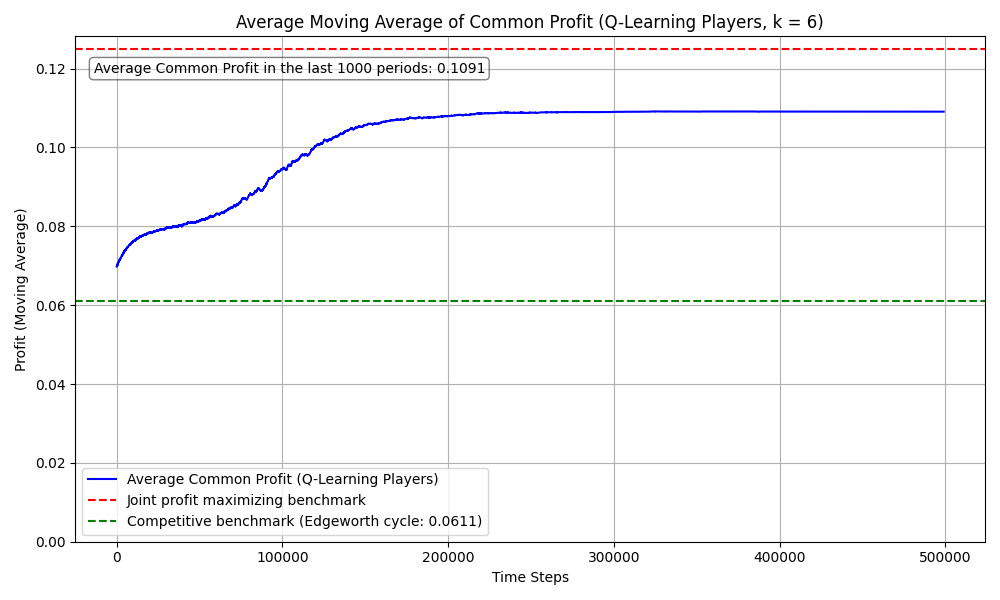
\includegraphics[width=\linewidth]{K=6.png}
        \caption{Q-learner vs Q-learner }
        \label{fig: K = 6}
    \end{minipage}
    \hfill
    \begin{minipage}{0.75\linewidth}
        \centering
        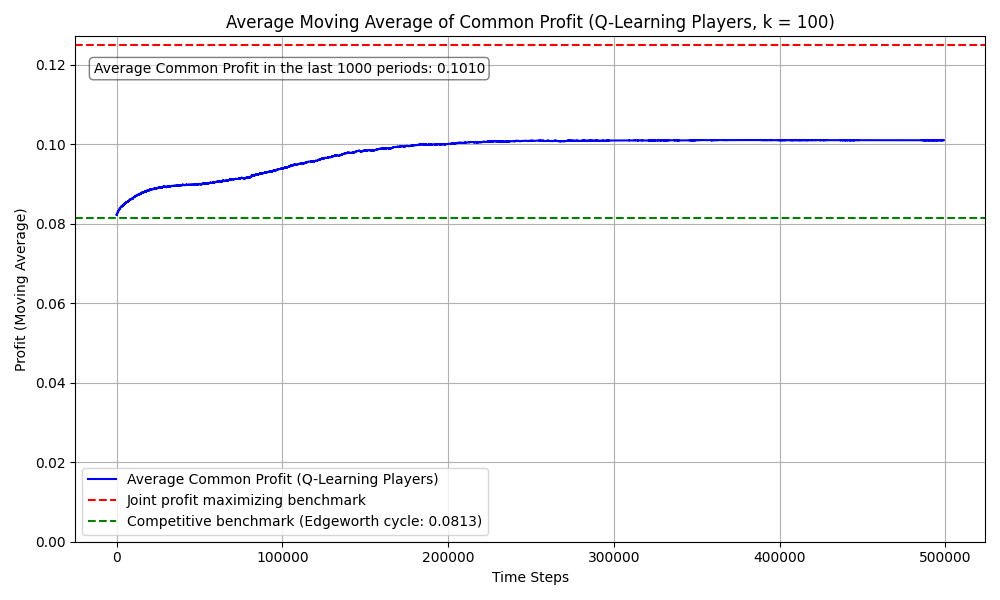
\includegraphics[width=\linewidth]{K=100.png} % Replace with your second image
        \caption{Q-learner vs Q-learner }
        \label{fig: K = 100}
    \end{minipage}
\end{figure}

\subsubsection{Random vs Random}
\label{RvsR}
Figure (\ref{fig: RANDOM K = 6}) and Figure (\ref{fig: RANDOM K = 100}) illustrate the simulation results for two random players interacting when $ k = 6 $ and $ k = 100 $, respectively. Corresponding results for $ k = 12, 24, 48 $ are included in the appendix. In these simulations, each player selects prices uniformly random when it is their turn, without any learning mechanism.
\newline
Unlike the Q-learning setting, these figures demonstrate an absence of learning, as evidenced by the flat path of average common profit (purple line) throughout the simulation. 
\newline
Although random players reach profit levels above the competitive benchmark, the magnitude of profit deviation from the benchmark is minimal compared to Q-learners. This underlines that the elevated profits in the Q-learning simulations are a result of adaptive behavior rather than random fluctuations.
\begin{figure}[H]
    \centering
    \begin{minipage}{0.75\linewidth}
        \centering
        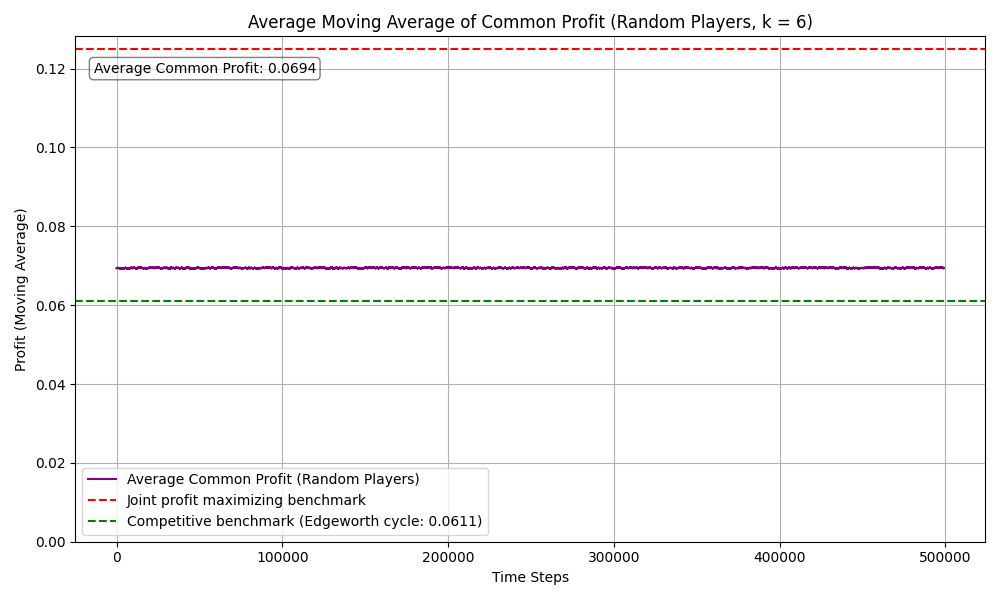
\includegraphics[width=\linewidth]{RANDOM PLAYER, K=6.png}
        \caption{Random players, k = 6 }
        \label{fig: RANDOM K = 6}
    \end{minipage}
    \hfill
    \begin{minipage}{0.75\linewidth}
        \centering
        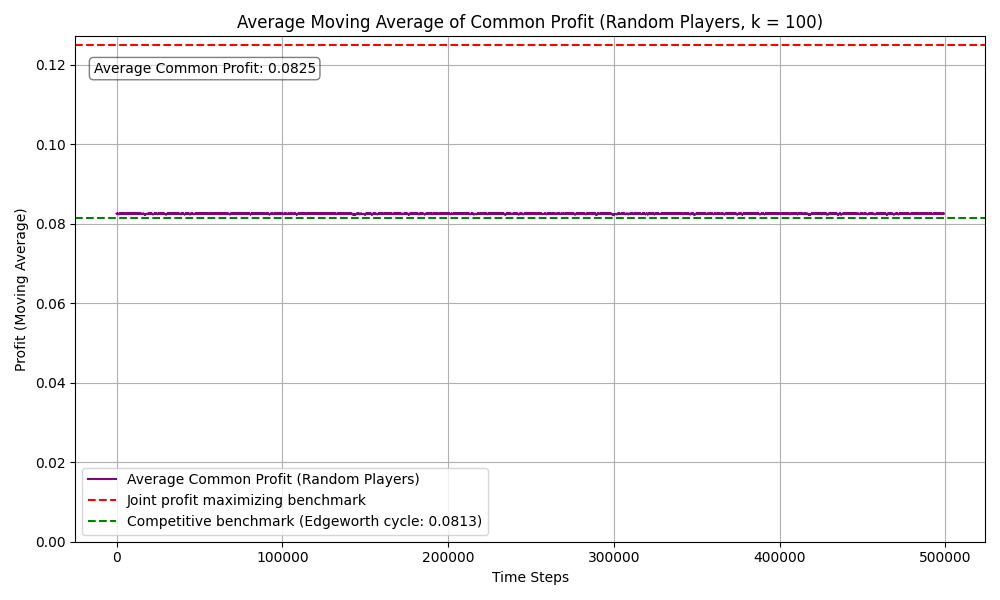
\includegraphics[width=\linewidth]{RANDOM PLAYER, K=100.png}
        \caption{Random players, k = 100}
        \label{fig: RANDOM K = 100}
    \end{minipage}
\end{figure}
\subsubsection{Level of Collusion for \textit{k} values}
\label{Level of Collusion for k values}
Table (\ref{tab:LevelCollusion}) presents the percentage deviation of the average profits calculated over the final 1,000 periods of each simulation from the respective competitive benchmark, across different values of the price interval parameter $k$. The table includes results for both Q-learners playing against Q-learners and random players playing against random players. Additionally, it reports the corresponding normalized collusion measure, $\zeta$, for each game. These results are derived from the simulations shown in Section \ref{QvsQ} and \ref{RvsR}. For instance, when $k = 6$, the Q-learners achieved an average profit that was 78.6\% above the competitive benchmark, with a corresponding $\zeta$ value of 75.1\%.
\begin{table}[H]
    \centering
    \begin{tabular}{|c|c|c|c|c|}
        \hline
        \textit{k} & \multicolumn{2}{c|}{\% deviation from Comp. benchmark} & \multicolumn{2}{c|}{$\zeta$}\\
        \hline
        & Q-learners & Random & Q-learner & Random \\
        \hline
        6 & 78.6 \%  & 13.6 \% & 75.1 \% & 13.0 \% \\
        \hline
        12 & 46.4 \% & 9.3 \%  & 58.8 \% & 11.8 \% \\
        \hline 
        24 & 39.2 \% & 5.4 \%  & 60.4 \% & 8.3 \% \\
        \hline
        48 & 36.6 \% & 2.9 \%  & 63.5 \% & 5.0 \% \\
        \hline
        100 & 24.2 \% & 1.5 \%  & 45.1 \% & 2.7 \% \\
        \hline
    \end{tabular}
    \caption{Illustrating the percentual deviation between the competitive benchmark and the average profit taken over the last 1000 periods for the Q-learners and the random players. In the last two columns we show the $\zeta$ values for corresponding k values.}
    \label{tab:LevelCollusion}
\end{table}
The results in Table (\ref{tab:LevelCollusion}) reveal what appears to be an inverse relationship between the parameter $k$ and the degree of collusive behavior observed. As $k$ increases, the average profit approaches the competitive benchmark for both Q-learners and random agents, indicating a reduction of the collusive level. This is intuitive: as the number of price choices increases, it becomes more difficult for agents to coordinate on supracompetitive prices and the moving target problem is intensified. 
For example, with $k = 6$, Q-learners achieve profits 78.6\% above the competitive benchmark, whereas at $k = 100$, this margin falls to just 24.2\%. This pattern persists across intermediate $k$ values (12, 24, 48), and also emphasizes the gap between the Q-learners and non-learners (random players).
\newline
The $\zeta$ values broadly confirm the overall trend that Q-learners exhibit decreasing levels of collusion as the price interval parameter \textit{k} increases. Specifically, $\zeta$ declines from 75.1\% at $k= 6$ to 45.1\% at $k=100$, indicating a shift toward more competitive behavior. However, this decline is not strictly monotonic across all reported values of $k$. We attribute these fluctuations to the underlying structure of the benchmark measures used in the $\zeta$ calculation. The competitive benchmark, is dynamic and varies with \textit{k}, whereas the collusive benchmark, defined by the joint profit-maximizing outcome, remains constant. As a result, observed profits move closer to the dynamic competitive benchmark as \textit{k} increases, while remaining at a relatively greater distance from the fixed collusive benchmark.
This can explain why the $\zeta$ values generally decline with \textit{k}, while exhibiting some variation between intermediate values.
The fluctuations could also be explained by simply not having done enough simulations, and the randomness associated with each run. The overall trend however is still clear, and shows a declining level of collusion from $k= 6$ to $k=100$.

\subsection{Characterization of Equilibrium Dynamics}
\label{Convergence Analysis}
In this section we will further investigate what happens when the Q-learning algorithms have converged towards their strategies. Therefore we will look closer at the prices that the different Q-learners are playing in the last periods, to detect if and what cycles arise, or if they end in focal pricing, where both firms repeatedly are setting the same price.

\subsubsection{Overview}
We have written Python code which detects price cycles when the algorithms have converged. We are looking at the last 1000 prices set by the two firms. We define a price cycle as a situation where two firms, having previously set the same set of prices against each other, return to that exact same set of prices after a sequence of price adjustments, thus repeating the same pattern of prices indefinitely. A full cycle starts at an initial set of prices and continues through subsequent sets of prices until returning to that same initial set of prices.
Notice that we are now investigating the prices set, instead of the profits that the firms are obtaining. 
\newline
For all values of \textit{k}, the shortest observed cycle length is 2. These instances are focal pricing and not cycles. However, they are identified as such, because of the sequential nature of the game. In this situation, both firms repeatedly set the same prices. We need to observe both firms setting their price. In step 1 firm i sets a price, which is then followed by step 2, where firm j sets a price, resulting in a 'cycle' of length 2.
\newline
As \textit{k} increases, the share of runs ending with focal pricing decreases. This trend can be seen in figure \ref{fig:ShareFocalPricing}. 
\begin{figure}[H]
    \centering
    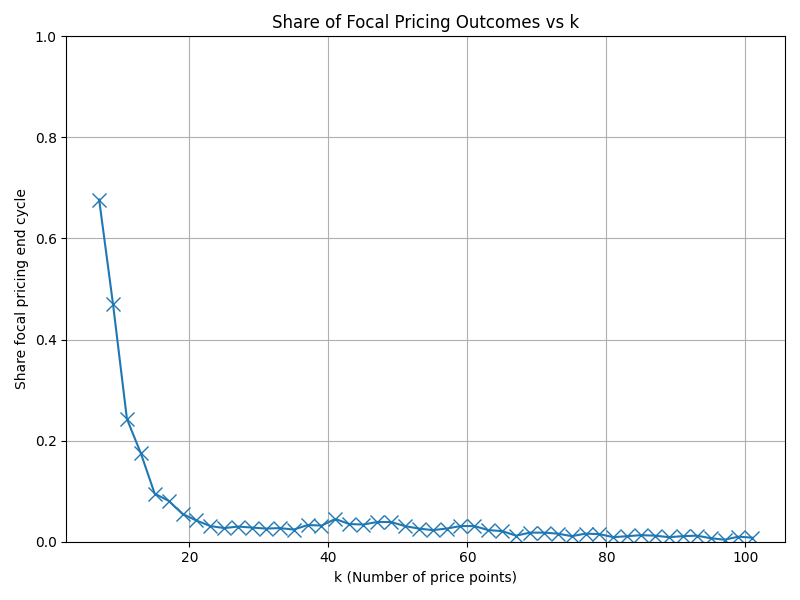
\includegraphics[scale = 0.5]{ShareFocal1000NumRuns.png}
    \caption{Share of focal pricing against \textit{k}}
    \label{fig:ShareFocalPricing}
\end{figure}
From Figure \ref{fig:ShareFocalPricing} it is clear to see that when $k = 6$, about 70 \% of the simulations end in focal pricing, whereas when k = 100 approximately 1 \% of the runs end in focal pricing. This trend shows that the firms have a harder time coordinating on setting the same price, and thereby ending in focal pricing, as the price interval, \textit{k}, grows.
\newline
The boxplots in figure \ref{fig:Boxplot} is a visualization of the distributions of end-cycle lengths. As already seen, as \textit{k} grows, the lengths of the cycles grows. This can be seen in both increases in the median and the mean. Furthermore, the longest cycle observed increases with \textit{k}. This is to be expected, as smaller price intervals will allow for more and longer price cycles.
\newline
plt.boxplot(data, labels=k_minus_1_labels, vert=True, showmeans=True, meanprops=meanprops)
DEFINER HVORDAN WHISKERSNE ER DEFINERET I BOXPLOTTET.

\begin{figure}[H]
    \centering
    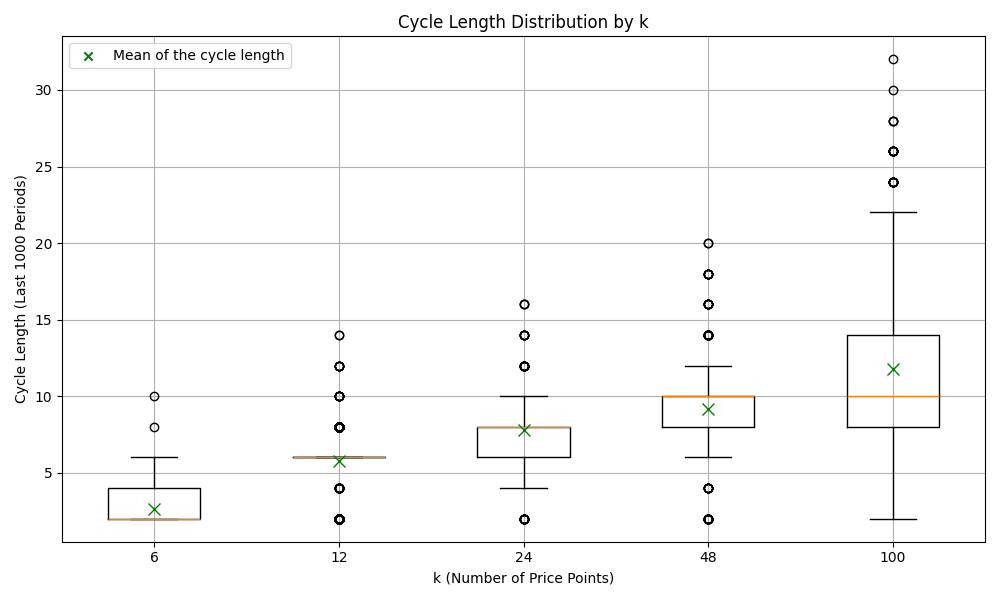
\includegraphics[scale = 0.5]{Boxplotv3.png}
    \caption{Boxplots for the distribution of the cycle lengths in the last 1000 periods for different values of \textit{k}. Notice the mean of the cycle length marked with a green x.}
    \label{fig:Boxplot}
\end{figure}


\subsubsection{In-depth look at cycles}
\label{In-depth look at cycles}
In this section we examine the specific pricing cycles that the algorithms converge to. As illustrated in Figure \ref{fig:Boxplot}, these cycles vary in length, and within each cycle length, multiple distinct cycles may occur. Due to the large number of observed cycles, we focus on two representative examples: one for $k = 6$ and one for $k=100$. To ensure representativeness, we selected the most frequently occurring cycle among those with lengths closest to the mean cycle length for each \textit{k} respectively, as shown in Figure \ref{fig:Boxplot}. For $k = 6$, although the mean is closest to a cycle length of 2, this reflects focal pricing rather than a price cycle. We therefore present a cycle of length 4. For $k = 100$, we present a cycle of length 12.
\begin{table}[H]
    \centering
    \begin{tabular}{|c|c|c|}
        \hline
        Step & price setting ($p_i$,$p_j$) &  profit ($\pi_i,\pi_j$) \\
        \hline
        1 & (\textcolor{red}{0.5},0.83) & (\textcolor{blue}{0.25}, 0.0)  \\
        \hline
        2 & (0.5,\textcolor{red}{0.33}) & (0.0, \textcolor{blue}{0.221}) \\
        \hline
        3 & (\textcolor{red}{0.167},0.33) & (\textcolor{blue}{0.139}, 0.0)  \\
        \hline
        4 & (0.167,\textcolor{red}{0.83}) & (\textcolor{blue}{0.139}, 0.0)  \\
        \hline
        Average Profit: & & (0.132, 0.055) \\
         \hline
        Average Common Profit: & & (0.0935) \\
         \hline
    \end{tabular}
    \caption{The most frequently observed four step cycle across 1,000 runs (29 occurrences) for k = 6. At each step, the red price indicates which firm sets the new price. Profits are shown, with blue marking the market winner. The final row presents average profits.}
    \label{tab:PriceCycleLen4}
\end{table}
In Table \ref{tab:PriceCycleLen4} we have the most frequently occurring four-step cycle which was observed 29 times across 1,000 simulation runs for $k = 6$. In this particular cycle, firm \textit{i} achieves a higher average profit per period than firm \textit{j} (0.132 compared to 0.055). However, an identical cycle in which the roles are reversed, where firm \textit{j} receives the higher profit, was observed 26 times. This near equal distribution of profit dominance suggests that while individual cycles may exhibit substantial differences in profit outcomes, these variations tend to balance out across repeated runs. Therefore, reporting the average profit across both firms (Average Common Profit), as we have done throughout the thesis, remains a meaningful and justified approach for summarizing overall performance.
\newline
We have extracted the final Q-matrices for firms \textit{i} and \textit{j} from the same simulation as Table \ref{tab:PriceCycleLen4}; these Q-matrices are available in Appendix \ref{Q-table}, as one combined Q-table. Based on the Q-table, we derive each firm’s Q-learned best response (QBR) functions, shown in Equations \ref{BR1-k6} and \ref{BR2-k6}.
\begin{equation}
    \label{BR1-k6}
    QBR_i(p_j)=\begin{cases}
        0 & \text{if $p_j$ $\in$ \{0, 0.167\}}\\
        0.167 & \text{if $p_j$ = 0.333}\\
        0.333 & \text{if $p_j$ = 0.5}\\
        0.5 & \text{if $p_j$ $\in$ \{0.667, 0.833, 1\}}\\
    \end{cases}
\end{equation}

\begin{equation}
    \label{BR2-k6}
    QBR_j(p_i)=\begin{cases}
        0.167 & \text{if $p_i$ = 0.333}\\
        0.333 & \text{if $p_i$ = 0.5}\\
        0.667 & \text{if $p_i$ $\in$ \{0.833, 1\}}\\
        0.833 & \text{if $p_i$ $\in$ \{0, 0.167, 0.667\}}\\
    \end{cases}
\end{equation}

These QBR functions explain the firms’ behaviour in the observed cycle by showing their learned optimal responses to competitor prices. 
\newline
In figure \ref{fig:QBR} we visualize these QBR functions.
\begin{figure}[H]
    \centering
    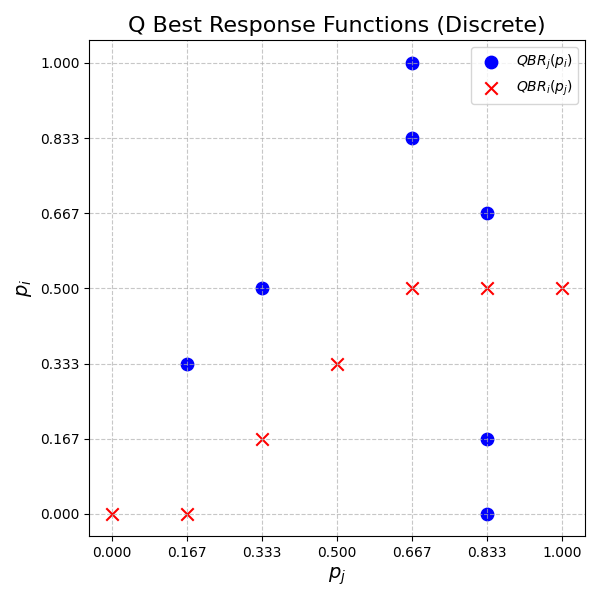
\includegraphics[scale = 0.5]{QBRgraph.png}
    \caption{Visualization of QBR functions from Equation (\ref{BR1-k6}) and (\ref{BR2-k6}).}
    \label{fig:QBR}
\end{figure}
Figure \ref{fig:QBR} directly shows us that it is not a Nash equilibrium. This is because none of the QBR points overlap, and therefore they are not best responding to each other. Furthermore the figures shows us that UNDERCUTTING BEHAVOIR FRA I OG OGSÅ DERFOR DEN VINDER SÅ MEGET?
\newline
Assuming the Q-matrices remain static, we also analysed whether any deviations could lead to different pricing cycles or focal pricing. From the functions \ref{BR1-k6} and \ref{BR2-k6} it is easily shown that no such deviations exist. For instance, if firm \textit{j} deviates by setting a price of 0.5:
\begin{align}
\label{CycleDeviationAndBackAgain}
    &QBR_i(0.5) = 0.333 \rightarrow QBR_j(0.333)=0.167 \rightarrow \\ &QBR_i(0.167) = 0 \rightarrow QBR_j(0) = 0.833\notag
\end{align}
Which leads back into the original cycle shown in Table \ref{tab:PriceCycleLen4}. Similar analyses for all other possible deviations for both firms yield the same result, confirming the stability of the cycle under the learned QBRs.
\newline
Given this stability, we now turn to the question of whether any deviation from the cycle could nonetheless be profitable for one of the firms. Specifically, we assess whether deviating from the learned (stable) strategy yields a higher expected profit than sticking to it, or whether the resulting sequence of punishments renders deviation unprofitable. If the cost of deviating outweighs the short term gain, this would further suggest tacit collusion, as a central feature of such behaviour is the ability to sustain high prices due to the expectation of a less profitable outcome following deviation( \cite{Klein2021}) (\cite{Calvano}). (DOBBELTTJEK DET HER). MÅSKE OMFORMULER LIDT I SIDSTE SÆTNING.
\newline
We have made the following table showcasing different expected averages for deviation within a specific step in the converged cycle shown in table \ref{tab:PriceCycleLen4}
\begin{table}[H]
    \centering
    \begin{tabular}{|c|c|c|c|c|}
        \hline
        Deviating price (\textcolor{blue}{p}) & \textit{i} deviates & \textit{i} deviates  & \textit{j} deviates & \textit{j} deviates \\
        \hline
         & (\textcolor{blue}{p},0.333) & (\textcolor{blue}{p},0.833)  &(0.167,\textcolor{blue}{p}) & (0.5,\textcolor{blue}{p}) \\
        \hline
        \textcolor{blue}{0} & \textcolor{red}{0.0} & \textcolor{red}{0.0}  & \textcolor{red}{0.0} & \textcolor{red}{0.0} \\
        \hline
        \textcolor{blue}{0.167}& \textcolor{orange}{in cycle} & \textcolor{green}{0.139}  & \textcolor{red}{0.023} & \textcolor{red}{0.046} \\
        \hline
        \textcolor{blue}{0.333} & \textcolor{red}{0.028} & \textcolor{red}{0.056} & \textcolor{red}{0.0} & \textcolor{orange}{in cycle} \\
        \hline
        \textcolor{blue}{0.5} & \textcolor{red}{0.0} & \textcolor{orange}{in cycle}  & \textcolor{red}{0.028} & \textcolor{red}{0.053} \\
        \hline
        \textcolor{blue}{0.667} & \textcolor{red}{0.111} & \textcolor{green}{0.222}  & \textcolor{red}{0.0} & \textcolor{red}{0.0} \\
        \hline
        \textcolor{blue}{0.833} & \textcolor{red}{0.083} & \textcolor{red}{0.107}  &\textcolor{orange}{in cycle} & \textcolor{red}{0.0} \\
        \hline
        \textcolor{blue}{1} & \textcolor{red}{0.083} & \textcolor{red}{0.083}  & \textcolor{red}{0.0} & \textcolor{red}{0.0} \\
        \hline
    \end{tabular}
    \caption{The average profit a firm can obtain by deviating with different prices from the (Q-learned) stable cycle, until it is back into the stable cycle again, just like shown in Equation (\ref{CycleDeviationAndBackAgain}). 
    Red numbers are cycles average profits which are lower than the average profit of the stable cycle they were already in. Green numbers corresponds to averages which are higher.}
    \label{tab:deviation averages}
\end{table}
Before analyzing Table \ref{tab:deviation averages}, recall that all possible deviations eventually return to the stable cycle shown in Table \ref{tab:PriceCycleLen4}.
We can see that if firm i deviates and sets its price at 0.667 when firm j has set its price at 0.833, its average profit from the corresponding deviation price cycle is $\pi_i=0.222$, which is higher than firm \textit{i}'s average profit from the stable cycle of $\pi_i=0.132$. This higher profit is the average for the deviation, and the steps up until it is back into the stable cycle again. 
\newline
By looking at the equations for the QBR's in ($\ref{BR1-k6}$) and (\ref{BR2-k6}) it is obvious that if firm i might be better off if it  changed its best response when $p_j = 0.833$ to $0.667$ instead of $0.5$. This would lead to a loop where the always set the price to: $(p_i,p_j) =(0.667,0.833)$ yielding an average profit for firm i to be $\pi_i (0.667,0.833) = 0.222$ and for firm j $\pi_j (0.667,0.833) = 0$.
\newline
However it is important to note that even though the current players have converged to a cycle, because epsilon have gotten to zero, this does not mean that if one player all of the sudden contentiously deviates, that the other player will not learn from this and change strategy to something which could harm the deivating firm. Even with no more exploration, the Q-tables would still get updated, for every move. Therefore it is to be expected that firm j would eventually change its strategy, after repeatedly getting profits of 0.
\newline 
Following the QBR's shown in equation \ref{BR1-k6} and \ref{BR2-k6}, firm i would set a price of 0.5, yielding a direct profit of 0.25 when responding to $p_j=0.833$. 
The Q-learnes does not have the ability to have 2 different actions for 1 state, because they play in pure strategies only making the original best response of 0.5 (direct profit 0.25) better and less costly than the deviation price of 0.667 (direct profit(0.222)) in the long run. 
\newline
For all of the above reasons, even though deviation does look more profitable, in the long run it could possibly not be more profitable, making it a short sighted move and not a longer run strategy. 
Because of the high $\delta$ value of $0.95$, the firms value future profit high, and this could be a reason for why firm \textit{i}, does not take the short term deviation.
\newline
The same analysis can directly be made with the other deviation position which looks more profitable in the short run for firm \textit{i} (where firm \textit{i} plays (0.167) to firms \textit{j}'s (0.833)). 
\newline
The fact that it is possible to deviate to end up with short term higher profits, but it is not done, is a sign of tacit collusion. If we recall, a key indicator for tacit collusion is that firms sustain high prices due to the fear of loss of profits in the long term (\cite{Klein2021} and \cite{Calvano}).


In table \ref{tab:CycleLen12} we have a randomly selected 12-step cycle across the 1,000 simulation runs for k = 100. The cycle length of 12 was chosen because this is the average cycle length the simulations ended up in when \textit{k}=100 (See \ref{fig:Boxplot}). 
\begin{table}[H]
    \centering
    \begin{tabular}{|c|c|c|}
        \hline
        Step & price setting ($p_i$,$p_j$) &  profit ($\pi_i,\pi_j$) \\
        \hline
        1 & (\textcolor{red}{0.340},0.420) & (\textcolor{blue}{0.224}, 0.0)  \\
        \hline
        2 & (0.340,\textcolor{red}{0.280}) & (0.0, \textcolor{blue}{0.202}) \\
        \hline
        3 & (\textcolor{red}{0.270},0.280) & (\textcolor{blue}{0.197}, 0.0)  \\
        \hline
        4 & (0.270,\textcolor{red}{0.140}) & (0, \textcolor{blue}{0.120})  \\
        \hline
        5 & (\textcolor{red}{0.910}, 0.140) & (0, \textcolor{blue}{0.120})  \\
        \hline
        6 & (0.910, \textcolor{red}{0.590}) & (0, \textcolor{blue}{0.242})  \\
        \hline
        7 & (\textcolor{red}{0.330}, 0.590) & (\textcolor{blue}{0.221}, 0.0)  \\
        \hline
        8 & (0.330, \textcolor{red}{0.240}) & (0, \textcolor{blue}{0.182})  \\
        \hline
        9 & (\textcolor{red}{0.120}, 0.240) & (\textcolor{blue}{0.106}, 0.0)  \\
        \hline
        10 & (0.120, \textcolor{red}{0.980}) & (\textcolor{blue}{0.106}, 0.0)  \\
        \hline
        11 & (\textcolor{red}{0.600}, 0.980) & (\textcolor{blue}{0.240}, 0.0)  \\
        \hline
        12 & (0.600,\textcolor{red}{0.420}) & (0.0, \textcolor{blue}{0.244})  \\
        \hline
        Average Profit: & & (0.091,0.093) \\
         \hline
         Average Common Profit: & & 0.092 \\
         \hline
    \end{tabular}
    \caption{An observed 12 step cycle across 1,000 runs for k = 100. At each step, the red price indicates which firm sets the new price. Profits are shown, with blue marking the market winner. The final rows presents average profits.}
    \label{tab:CycleLen12}
\end{table}
In Table \ref{tab:CycleLen12} we see a cycle with no clear dominant firm. Even though firm \textit{j} achieves a slightly higher average profit, the outcome is arguably balanced. Unlike the cycles observed for $k =6 $, both firms take turns resetting the cycle, after undercutting each other: firm \textit{i} increases its price to 0.910 at step 5, and firm \textit{j} resets at step 10 by raising its price to 0.980. This pattern resembles an Edgeworth cycle, however just not the most competitive one. Both firms obtain average profits exceeding the per period profit of the most competitive Edgeworth benchmark ($0.092$ compared to $0.081$). A key reason for this is that the firms reset the cycle before prices reach marginal cost (0), indicating that they have learned to sustain more profitable strategies than the most competitive Edgeworth cycle.
 
\section{Discussion}
Our simulations confirms the findings of \cite{Klein2021} by demonstrating that algorithmic collusion can occur. However, the extent of collusion varies depending on the parameter, \( k \), which determines the number of possible prices in the Q-learning environment. The parameter \( k \) plays a crucial role in shaping the equilibrium dynamics: a lower \( k \) typically results in shorter cycle lengths, which typically results in more collusive behavior. In contrast, higher values of \( k \) increase the size of the action space, leading to longer price cycles and generally resulting in a reduced degree of collusion.

As \( k \) increases, we observe a lengthening of undercutting phases within the price cycles, which then reduces the average profit obtained by the firms, for instance, from \( k = 6 \) to \( k = 100 \), average profits decline. This could suggest that coordination becomes increasingly difficult as the number of pricing options expands. Intuitively, a finer price grid introduces greater complexity to the environment, worsening the moving target problem and making it harder for the algorithms to identify and sustain supra competitive prices. Moreover, since the number of Q-values that must be learned grows with \( k \), parameters that are calibrated for low \( k \)-values like \( k = 6 \) may no longer yield optimal performance in environments with larger action spaces such as $ k = 100$.
(CHAT OVENOVER)
\newline
We evaluated the algorithms in the end of the runs after convergence. However, the convergence observed might not reflect learning of an equilibrium strategy but rather
convergence due to the decay of the exploration rate, $\epsilon$. We justify the approach of still saying the algorithms have converged, by the fact that the convergence happens after a period of learning in the beginning. Furthermore, the cycle we examined extensively showed that no possible deviations could throw it out of the cycle, and thus the cycle was stable. It is not unreasonable to assume that other cycles in other runs are also stable, because of the flattening of the profit curve towards the end. (See Figure (\ref{fig: K = 6}) and (\ref{fig: K = 100})) 
\newline
Diving into a specific converged cycle for k = 6, we investigated the dynamics further, and found more evidence of collusive and egdeworth-alike cyclical behaviour. This was seen in the way that one firm had a chance to undercut, which would give more profit in the short term, but choose not to, which is a typical sign of collusive behaviour (\cite{Klein2021}, \cite{Calvano}).
\newline The cyclical pricing behavior we observe for different k-values is supported by empirical evidence from a study by \cite{Noel2007}. Noel documents price cycles in Toronto’s gasoline market that closely resemble Edgeworth cycles, which is something we also noticed in our simulations for the cycle of length 12 when k = 100. This empirical correspondence suggests that the cycles generated by our model are not purely theoretical but may help to depict realistic pricing dynamics observed in actual markets.
\newline
Additionally, the cyclical pricing observed in our simulations, could be held up against the empirical findings in the work of \cite{LEON2024}. He analyzes pricing data from Amazon Marketplace and finds that automated pricing algorithms can induce tacit collusion through strategies that periodically reset prices to encourage competitors into raising theirs. These observed pricing cycles also resemble Edgeworth cycles, and his model suggests that such algorithmic based price setting can maintain average prices close to monopoly levels. This supports the idea that the cycles we see in our Q-learning simulations illustrates behavior which is possible and exists to some degree in modern digital markets. 
\newline
Further, \cite{Assad} studied the german gasoline market, and found empirical evidence that supported that the adoption of algorithmic pricing at gas stations increased profits. They found that in a duopoly setting, if both stations adopted algorithmic pricing, margins increased by 28\%. 
These studies underline the validity of using a simulation approach, as the findings are supported empirically, both in terms of collusion and the pricing patterns (cycles).
\newline
Due to the fact that the parameters used might be specificially chosen to the k = 6 Q-learner, which shows more collusive behaviour, this could indicate that the reason for K = 100 showing less collusive behaviour is to the facts that the parameters is not fine tuned for  k=100. Further more this could then indicate that the parameters and therefore the simulations study introduced by klein from the beggining was set up to fail, meaning, setup to be collusive. 
\newline
But keeping this in mind one we would argue that this thesis should be based on the best version, and therefore most optimal chosen parameters, to be representative of how Q-learner would act. The algorithm is not being punished for playing collusive.  
\newline
In our simulations our economic environment is static and simplified version of a real world scenario. Our profits and thereby demand functions remains the same and does not adjust accordingly, as it would in the real world. Consequently, the behavior of learning algorithms in this static environment might differ from how they would perform in a more complex and adaptive market. \cite{Klein2021} also brings this to light by saying that the economic environment is quiet stylized and that Q-learning algorithms would find it increasingly difficult if the environment were more complex.
\newline 
One may ask, how realistic is a k value of 6, and thereby a pricegrid where firms can only set 7 different prices? The answer is that it depends on the good. For gasoline markets, a k value of 6 is not very realistic compared to a k value of 100. Gasoline prices typically change with very small increments (in sizes as small as cents (\cite{eia_gasoline_fluctuations})), making a higher k value more realistic as this makes a finer price grid. Whereas a good like butter typically would not fluctuate as much in price, and a less fine price grid would be more accurate in this setting. However whatever the good, and corresponding k value which would be most realistic, our simulations show that algorithmic pricing collusion is happening.
\newline
Q-learning is a simple reinforcement learning algorithm, and one can imagine that firms 'in the real world', would use more advanced algorithms. This is exactly what the paper from \cite{Julius2023} looked into. He used Q-learning, as well as more sophisticated reinforcement learning algorithms to check for the possibility of collusion. His findings confirmed that more advanced algorithms also learn to behave collusively. 
\newline
Collusive behaviour hurts the consumers. Therefore collusion is illegal. However, the collusion that we are observing in our simulations is on the form of tacit collusion. This mean that the algorithms are reaching collusive outcomes, without communicating. In general, collusion is difficult to detect, because the agents involved wants to keep it a secret. When speaking of tacit collusion it is even more difficult to discover and prove, as there is no explicit communication as evidence. 
However policy makers still have tools to combat this tacit collusion arising from algorithmic pricing. \cite{Asker} also dived into algorithmic pricing, and they differentiated between two different forms of Artificial Intelligence Algorithms; namely asynchronous and synchronous learning. The first is when the algorithms only learn from the paths and choices which they take, and is comparable to our setting. They found that algorithms in this setting leads to pricing close to monopoly level. However, they also investigated synchronous learning, where algorithms not only learn from the path they take, but also from the paths they dont take, and found that this type of learning leads to pricing at the competitive level.
Therefore, an idea for a policymaker to combat the problem of collusive algorithmic pricing could be to demand users of algorithmic pricing, to use synchronous learning. However the implementation of this could prove to be difficult.
\newline
COMPETITVE BENCHMARK METRICS
\section{Conclusion}
From this thesis we could conclude that ... 





\newpage 
\section{References}

\bibliographystyle{apalike}
\bibliography{references}


\section{Appendix}
\subsection{Q-learning collusion graphs}
\subsubsection{ Definition 2 - Stochastic Game}
\label{stochasticgamedef}
\textbf{Definition 2 (Stochastic game)\citep[p. 47-48]{marl-book}} A stochastic game consists of:
\begin{enumerate}
    \item Finite set of agents \( I = \{1, \dots, n\} \)
    \item Finite set of states \( S \), with a subset of terminal states \( \bar{S} \subset S \)
    \item For each agent \( i \in I \):
    \begin{itemize}
        \item Finite set of actions \( A_i \)
        \item Reward function \( R_i: S \times A \times S\to \mathbb{R} \), where \( A = A_1 \times \dots \times A_n \)
    \end{itemize}
    \item State transition probability function \( T: S \times A \times S \to [0, 1] \) such that
    \[
    \forall s \in S, a \in A : \sum_{s' \in S} T(s, a, s') = 1
    \]
    \item Initial state distribution \( \mu: S \to [0, 1] \) such that
    \[
    \sum_{s \in S} \mu(s) = 1 \quad \text{and} \quad \forall s \in \bar{S}: \mu(s) = 0
    \]
\end{enumerate}
\subsubsection{k = 12}
\begin{figure}[H]
    \centering
    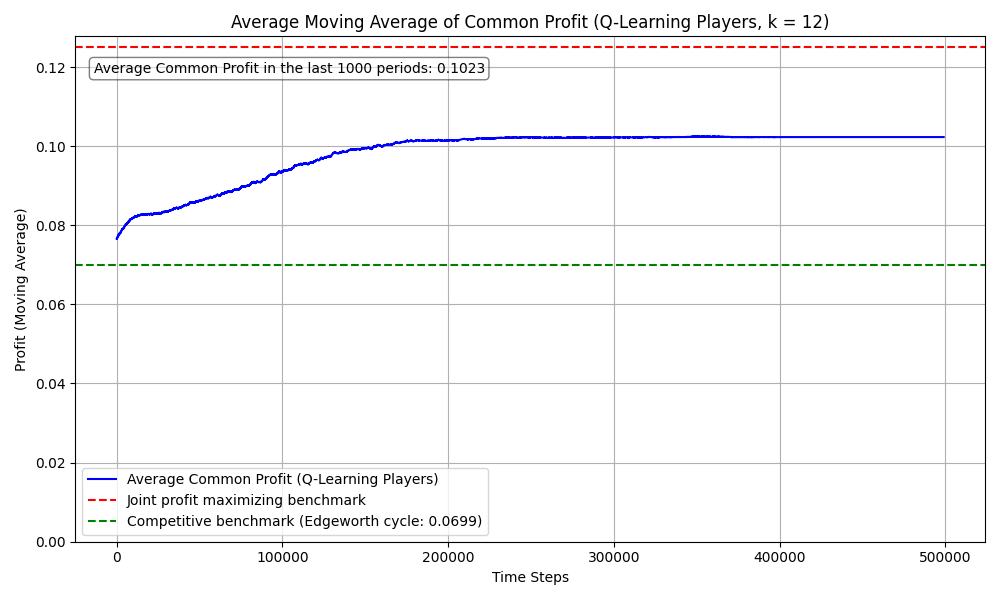
\includegraphics[scale = 0.45]{K=12.png}
    \caption{Q-learner vs Q-learner when k = 12}
    \label{fig: QlearnervQlearnerK=12}
\end{figure}

\subsubsection{k = 24}
\begin{figure}[H]
    \centering
    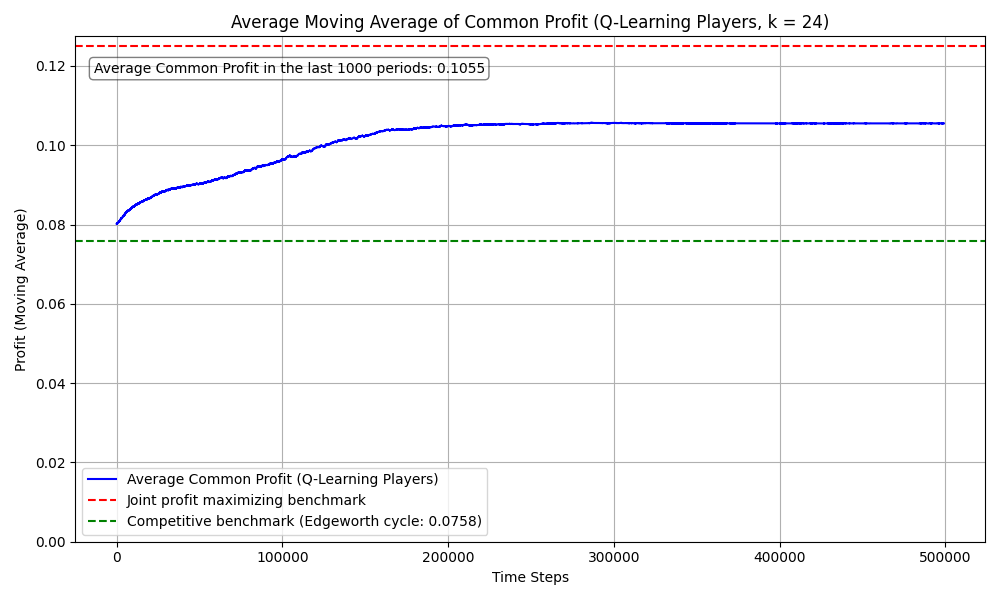
\includegraphics[scale = 0.45]{K=24.png}
    \caption{Q-learner vs Q-learner when k = 24}
    \label{fig: QlearnervQlearnerK=24}
\end{figure}

\subsubsection{k = 48}
\begin{figure}[H]
    \centering
    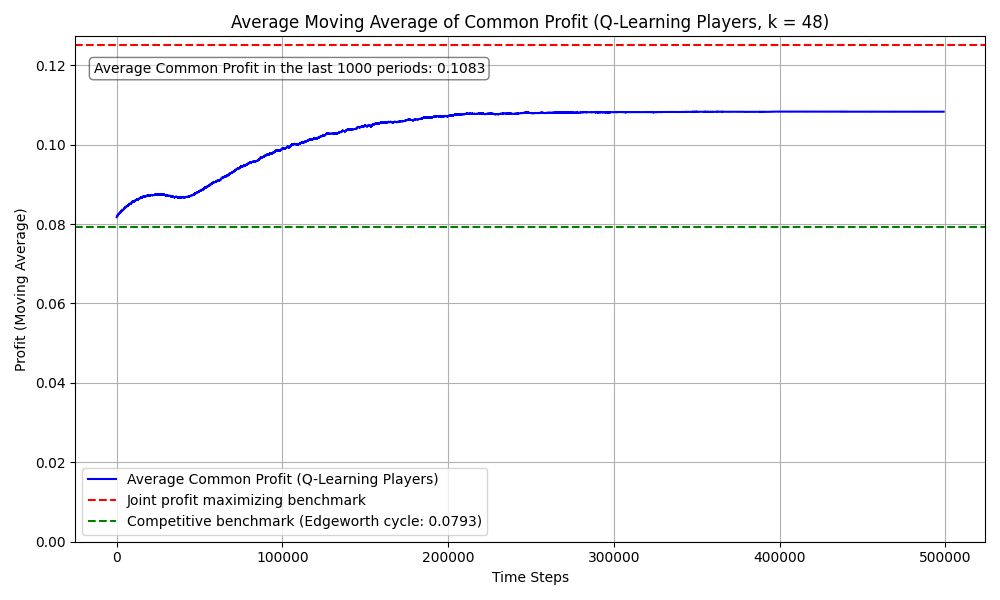
\includegraphics[scale = 0.45]{K=48.png}
    \caption{Q-learner vs Q-learner when k = 48}
    \label{fig: QlearnervQlearnerK=48}
\end{figure}
\subsubsection{Q Matrix - cycle length 4 -  k=6}
{\scriptsize
\[
\begin{array}{c|@{\hskip 5pt}c@{\hskip 5pt}c@{\hskip 5pt}c@{\hskip 5pt}c@{\hskip 5pt}c@{\hskip 5pt}c@{\hskip 5pt}c}
 Q  & \overbrace{s_1}^{p=0} & \overbrace{s_2}^{p=0.167} & \overbrace{s_3}^{p=0.333} & \overbrace{s_4}^{p=0.5} & \overbrace{s_5}^{p=0.667}& \overbrace{s_6}^{p=0.833} & \overbrace{s_7}^{p=1} \\
\hline
a_1 & \textcolor{blue}{2.361}, 1.054 &\textcolor{blue} {2.398}, 1.014 & 2.289, 1.078 & 1.323, 0.999 & 2.132, 1.662 & 1.365, 1.503 & 1.763, 1.645 \\
a_2 & 1.212, 1.061 & 1.197, 1.058 & \textcolor{blue}{2.676}, \textcolor{red}{1.142} & 1.308, 1.153 & 2.013, 1.564 & 2.051, 1.596 & 1.986, 1.525 \\
a_3 & 1.165, 1.074 & 1.191, 1.010 & 2.275, 1.113 & \textcolor{blue}{2.442}, \textcolor{red}{1.198} & 1.706, 1.621 & 2.125, 1.599 & 1.618, 1.627 \\
a_4 & 1.098, 1.061 & 1.185, 1.037 & 2.227, 1.101 & 1.331, 1.149 &\textcolor{blue}{ 2.665}, 1.673 & \textcolor{blue}{2.665}, 1.568 & \textcolor{blue}{2.665}, 1.627 \\
a_5 & 1.483, 1.078 & 1.195, 1.062 & 2.404, 1.112 & 1.319, 1.110 & 2.098, 1.583 & 1.991, \textcolor{red}{1.609} & 1.874, \textcolor{red}{1.691} \\
a_6 & 1.213, \textcolor{red}{1.093} & 1.194, \textcolor{red}{1.081} & 2.235, 1.117 & 1.327, 1.087 & 1.947, \textcolor{red}{1.726} & 2.255, 1.606 & 1.912, 1.621 \\
a_7 & 1.212, 1.076 & 1.166, 1.052 & 2.202, 1.119 & 1.320, 1.103 & 1.844, 1.609 & 2.105, 1.483 & 1.868, 1.603 \\
\label{Q-table}
\end{array}
\]
}
\begin{center}
    Matrix 1: Final Merged Q-matrices ($A\times S$) for firm i and j, from the K=6 run, shown in table \ref{tab:PriceCycleLen4}. Each entry in the matrix is the tuple of Q-values from firm i and j ((1,1) = ($(Q_i(a_1,s_1),Q_j(a_1,s_1)) =(2.361 , 1.054) $).
    The Blue corresponds with firm i's maximizing action in that given state (competitor price) and red the same for firm j. It can be read as follows. If the state was $s_5$, (a competitor price of 0.667 (column 5)), firm i responds with action $a_4$ (setting a price of 0.5), since 2.665 is the highest Q-value for that given state/column. Given the same state firm j would respond with $a_6$ (setting a price of 0.833). This is when their actions are solely based on their learned Q-matrix, and thereby maximizing the Q-value given a state, which is how it would be at the end of the simulations as exploration. 
\end{center}

\end{document}
